\chapter{Methodology}
% information on the corpus and writing data
%define  features that I will use for classification how I decided on this and motivation behind these features.

\section{Characteristics of Japanese}
talk about about Japanese text is processed in regards to how it will be treated for my analysis
   Kanji vs. Hiragana, - since dealing with learner texts, the lower learners have a preference for hiragana so this
is taken into consideration when matching grammatical forms. - for the most part the tokenizer seems to be able to
still parse when using only hiragana - but of course spelling errors can through this off. However the system will
most likely not be robust againast "spelling" errors or errors using mistaken kanji.

What is considered a word in Japanese may differ from other languages. In English, a bound morpheme may be treated as an individual word; however, this is not the case in Japanese. For example, the word 話す\textit{hanasu}(to speak) would be considered one word, but the potential form 話せる \textit{hanaseru}(to be able to speak) would be considered two separate words consisting of \textit{hanas} and \textit{eru}.

\section{About the International Corpus of Japanese as a Second Language(I-JAS)}
information about the IJATS corpus organization, prepossessing,

This study utilizes data from the International Corpus of Japanese as a Second Language (I-JAS), as detailed in \citet{Sakoda2020}.  The I-JAS corpus includes both spoken and written samples of Japanese from a diverse pool of 1,000 adult learners aged between 17 and 63 years, all of whom are learning Japanese as a second language. 50 Native speaker samples are also included in the corpus.

To assess each participant's proficiency level, the Japanese Computer Adaptive Test (J-Cat) by \citet{Imai2009} was administered. Further information about this test, including its scoring methodology, is provided in the subsequent section. In addition to language proficiency data, various metadata, such as participants' native language, prior experiences of visiting or living in Japan, and current location (whether outside or within Japan), were also recorded.

%%%%%%% This part below contains information only on the essay writing samples I previously analyzed. I have also
%%%%%%% included additional writing samples added to the corpus which has brought the total particiapnt pool to 1000
%%%%%%% again.
From the larger pool of participants, writing samples were obtained from 687 individuals, including a control group
of 50 native speakers. A breakdown of the proficiency groups among these 687 participants who submitted writing
samples is presented in Table 1.

%need to update this table to account for JLPT levels, N5, N4, N3, N2, N1.

%JLPT
%N5    176
%N4    318
%N3    297
%N2    165
%N1     44
%NS     50

Name: count, dtype: int64
\begin{table}
\centering
\begin{tabular}{cc}
\hline \textbf{JLPT Proficiency Level} & \textbf{\# of Participants} \\ \hline
N5 & 176 \\
N4  & 318 \\
N3 & 297\\
N2 & 165 \\
N1 & 44 \\
Native & 50 \\
\hline
\end{tabular}
\caption{\label{participants-chart} breakdown of participants per proficiency level}
\end{table}


\subsection{J-CAT test}

%background and information on the J-CAT test compare to JLPT.

The J-Cat, short for Japanese Computerized Adaptive Test \cite{Imai2009}, is a computer-administered assessment that
evaluates an
individual's proficiency in the Japanese language. The test used to be offered freely to lerners of Japanese however
it is now currently overseen by the 日本語教育支援協会(Japanese Language Education Support Association (JaLESA)) , Japanese
universities widely
employ this test as an efficient tool for assessing the language skills of foreign students seeking placement in
Japanese language courses, as it can be adminsitered anytime during the year, as opposed to the JLPT which is only
administered bi-annualy. This adaptive test tailors its
question difficulty to a
student's performance in
the areas of Vocabulary, Grammar, Listening, and Reading.

\begin{figure}[h]
    \centering
    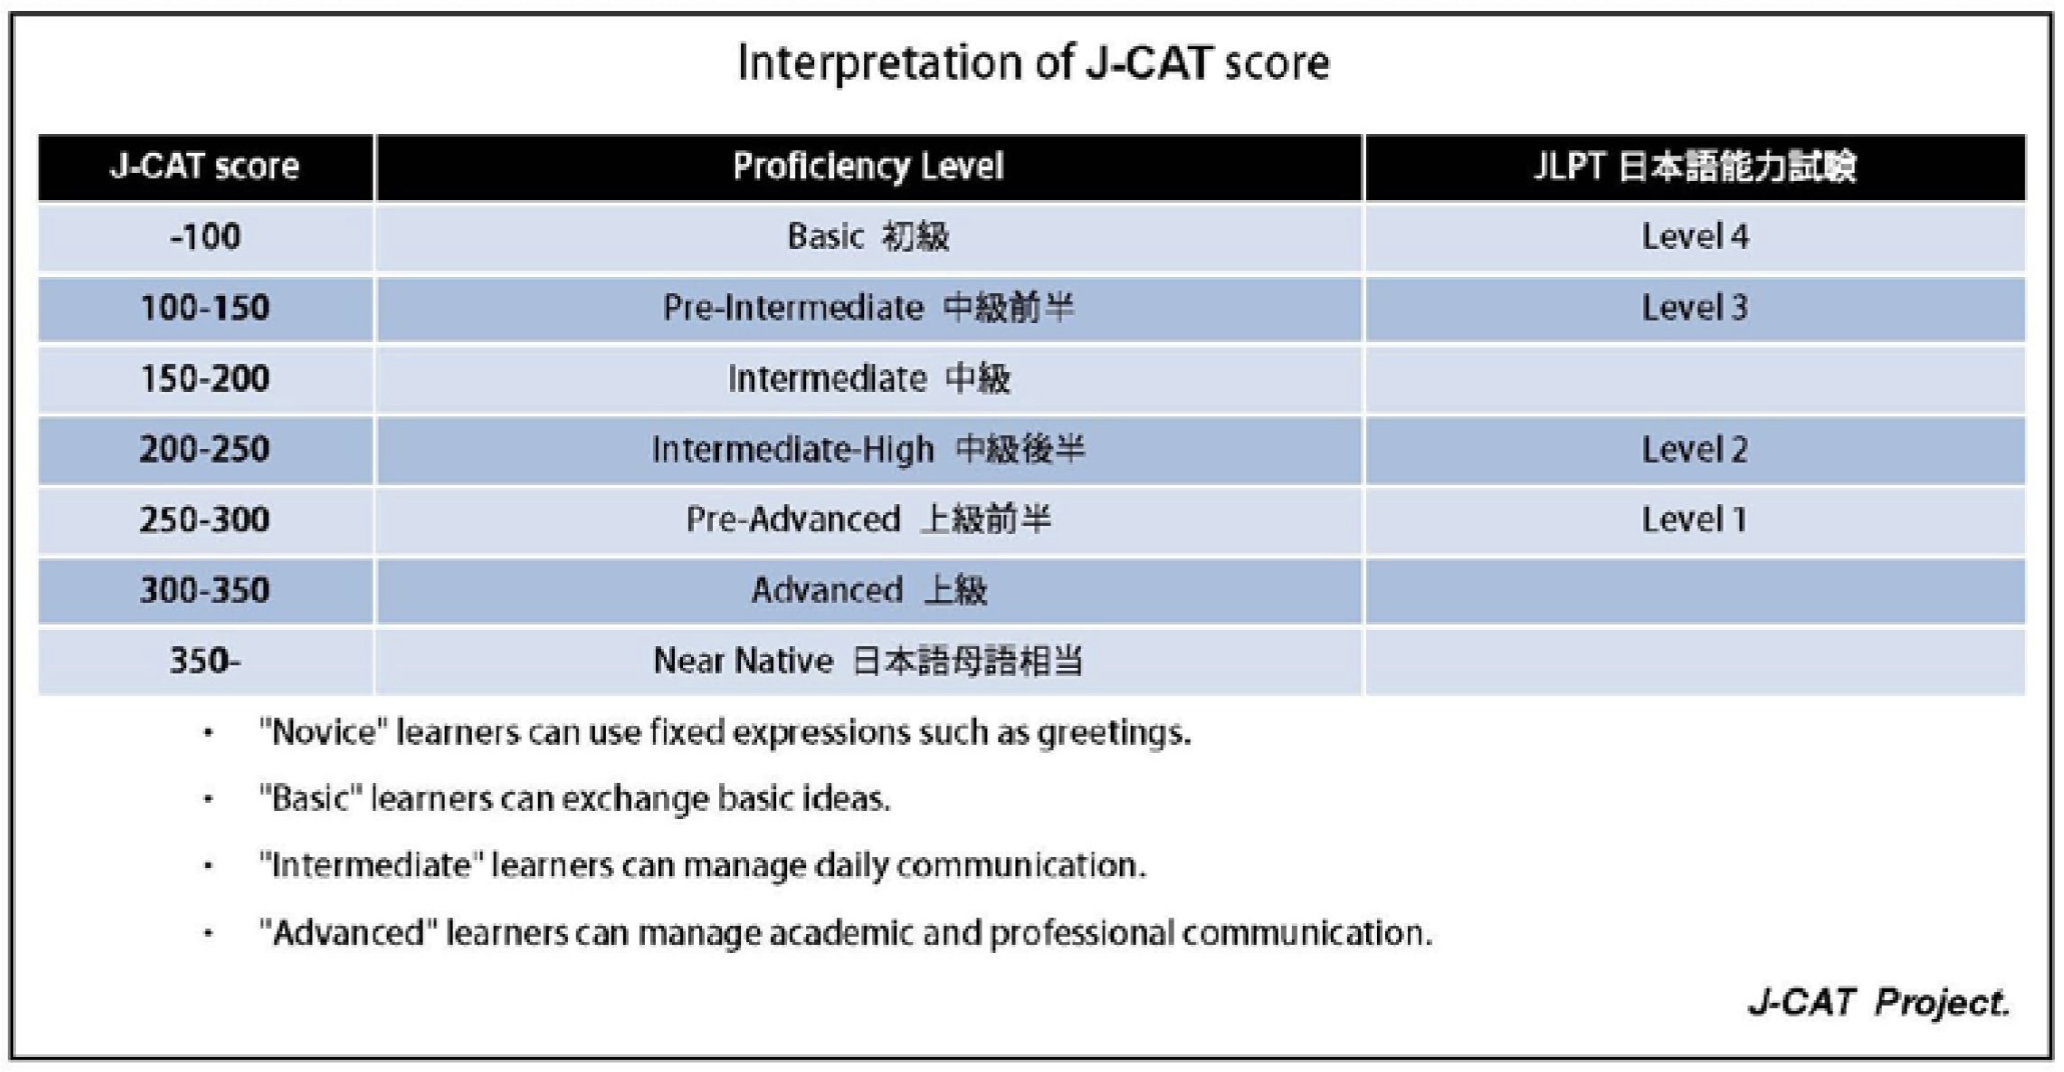
\includegraphics[scale=.3]{img/JCatScores.png}
    \caption[J-Cat Proficency Levels]{The assigned proficency levels from the J-Cat test as taken from the original paper in  2009. Please note that the given JLPT levels do not correspond to the current JLPT test which was reformed in 2010. A new score interpretation connecting JLPT levels to J-Cat scores was released in 2011 and is shown in Table \ref{tab:proficency-table} }
    \label{fig:JCatLevels}
\end{figure}

Each student receives a numerical score that corresponds to one of seven distinct proficiency levels, as detailed in
Table \ref{tab:proficency-table}. This study will categorize participants according to their J-Cat proficiency level. Participants in the
native speaker control group were given a default J-cat score of 999.

\begin{table}
\centering
\begin{tabular}{lrl}
\hline \textbf{JLPT Proficiency Level} & \textbf{J-Cat Score}  \\ \hline
N5 & 0 - 149 \\
N4 & 150 - 199 \\
N3 & 200 - 249 \\
N2 & 250 - 299 \\
N1 Pre-Advanced & 300 + \\
\hline
\end{tabular}
\caption[Proficency Levels]{Proficency level classification based on J-cat score taken from \cite{jcat_interpretation_guide}.}
\label{tab:proficency-table}
\end{table}

\subsection{Writing Tasks}

% add the additional SW 1 and 2 tasks where participants were expected to write a story based on a picture.
Each participant submitted four samples of writing for specific tasks:
\begin{itemize}
    \item A short essay titled "Our Eating Habits" involving a comparison between fast food and home-cooked meals in the learner's home country.
    \item A letter addressed to a former teacher, requesting a letter of recommendation for a scholarship application.
    \item An email seeking an extension for the deadline of a report submission.
    \item An apology email in which the learner must decline an invitation.
\end{itemize}
These tasks were consistent across all participants, regardless of their proficiency levels, and encompassed various
task types. The inclusion of a range of task types and formalities was intended to encourage diverse responses from
the students and possibly mitigate a potential "task effect" similar to what  was described in \cite{Alexpoulou2017}.
The writing samples were processed-as-is without being corrected for learner errors.

\section{Complexity Measures}
detail the complexity measures I will use, how I developed the scripts to automatically "extract them" and the statistical significance between the proficiency levels
list, Sent Length, Clauses per sentence, Noun phrase length,  Subordination, coordination, noun phrase length, MTLD,Morphological complexity? , ADD measures?

lexical sophistication measures use this corpus: \cite{BCCWJ_List} and article citation: \cite{maekawa2014}, Think
about the Tsukuba web corpus also...
When implementing LFP punctuation is removed from the text. Need to mention how text is tokenized in japanese: in
the freq list ばいい is written but would be tokenized as ば and いい ...how to overcome this? Remove verbs? should I use
tokenizer to split the verbs in the word list??

mention the difficulties in finding clauses - specifically in discriminating between coordinate and subordinate
automatically.  POS label SCONJ for subordinate conjunction is used even in the case of coordination, therefore
other methods are needed.

\section{Criterial Features}
Describe the rule based feature matcher I made for extracting certain grammar patterns to disconcern their use
across proficiency levels. Mention how many grammar points at each level I was able to include. Use of the lower
levels doesn't disconcern much so focus should be on the intermediate and upper levels.  Forms that are mainly form
based(and therefore easier to pattern match) should be given priority over. Give some examples of rules derrived

mention that I chose forms which spanned multiple levels. I.e. しか at N4 used with Nouns and しか〜ないat N3 used
with verbs to see if their use at the different levels actually follows this.

don't forget about implementing normalization.

Official documents with grammar from the different levels of JLPT do not exist however many 'unoffical lists' of
grammar, vocabulary, Kanji are available - including Jisho.org, personally compared againast published material from
ARUKU

\section{EBMS}
 Here I will give a brief overview of Explainable boosting machines and why I chose them for my analysis.


